\chapter{Overview of the \texorpdfstring{$\text{M}_\text{T2}$}{MT2} Analysis}

Physics beyond the Standard Model at the LHC may manifest itself in a wide variety of potential final state 
topologies. Phase space covering a wide range of the relevant kinematic variables, such as hadronic energy,
missing transverse momentum, and number of leptons, should be carefully searched for signs of new physics.
In this dissertation, we focus on the ``all-hadronic'' final state,
which encompasses events with no prompt leptons and large amounts of hadronic energy and missing transverse momentum.
Section~\ref{sec:motivation} discusses the theoretical motivation for an all-hadronic search, Sec.~\ref{sec:mt2_backgrounds}
describes the various backgrounds for such a search, and Sec.~\ref{sec:mt2_variable} introduces \mttwo, a \ptmiss-based kinematic
variable that is used to discriminate signal from background.

\section{Motivation for an all-hadronic search}
\label{sec:motivation}

Many theories of BSM physics contain heavy particles (masses on the order of hundreds of GeV to TeV), whose
decays produce a multitude of highly energetic particles. Thus, the events tend to have lots of visible
energy (in the form of highly energetic jets and/or leptons) as well as
\emph{invisible} energy (in the form of \ptmiss), if the decay products are not detectable.

Most SM processes that produce significant true \ptmiss from neutrinos also have leptons, since the
neutrinos often come from $W\to\ell\nu$ decay. This is especially true for events with many jets
and b-tagged jets, which often contain a \ttbar pair. So by vetoing events with prompt leptons, it is
possible to significantly reduce a large class of SM backgrounds. The flip side of this is that a
zero-lepton selection will be contaminated by events from QCD multijet production, with significant
fake \ptmiss from jet mis-measurement. However, this can be managed with the use of a variety of
discriminating kinematic variables, discussed in Sec.~\ref{sec:mt2_variable} and Chapter~\ref{chap:event_selection}.

Based on general concerns, then, there is motivation for a search with lots of hadronic energy and
missing transverse momentum, but no leptons. There are also many specific examples of models
of BSM physics that produce such final states. Decay chains in simplified models of supersymmetry, discussed in
Sec.~\ref{sec:susy}, are often completely hadronic. Two examples are shown in Fig.~\ref{fig:example_susy_feyn}.
The left diagram shows the pair production of two gluinos, each decaying to a \ttbar pair and an invisible \lsp.
Each top quark then has a 68\% probability of decaying purely hadronically. The right diagram shows
the pair production of bottom squarks, each of which decay to a bottom quark and \lsp.

\begin{figure}[t]
  \begin{center}
    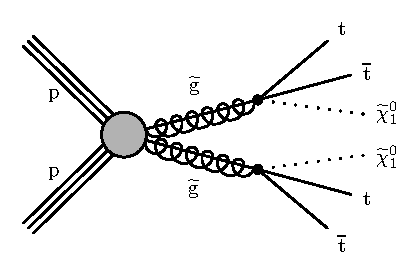
\includegraphics[width=0.40\textwidth]{figs/susy_diagrams/T1tttt.pdf}
    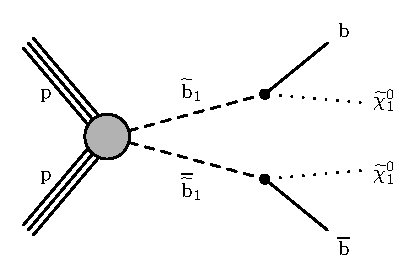
\includegraphics[width=0.40\textwidth]{figs/susy_diagrams/T2bb.pdf}
    \caption{Example Feynman diagrams of strongly-produced SUSY particles decaying hadronically.
      (left) Gluino pair production, where each gluino decays into a neutralino and two top quarks.
      (right) Bottom squark pair production, where each squark decays into a neutralino and bottom quark.
            }
    \label{fig:example_susy_feyn}
  \end{center}
\end{figure}

Additionally, the pair production of leptoquarks, discussed in Sec.~\ref{sec:leptoquarks}, may produce purely hadronic final
states if each leptoquark decays into a quark and neutrino (e.g., $\mrm{LQ}\to t\bar{\nu}_\tau$). In the case that the
leptoquarks are scalars (spin 0), this process is indistinguishable from the pair production of squarks that decay to a quark 
and \lsp when $m_\lsp=0$, so any analysis optimized to search for hadronically-decaying squark pairs is naturally optimized
to search for leptoquark pairs.


\section{Sources of backgrounds}
\label{sec:mt2_backgrounds}

The \mttwo analysis targets new physics signatures in all-hadronic events with large amounts of missing transverse momentum.
This selection leads to backgrounds that fall into three main categories:
\begin{enumerate}
\item \textbf{Invisible Z}: \znunu events produced in association with jets contain genuine \ptmiss, and represent
an \emph{irreducible} background to the analysis. While there is no real handle to eliminate these events, as they
look exactly like signal, the events contain no inherent b jets so the background becomes less important in
signal regions with large numbers of b-tagged jets. This background is estimated using \zll events,
as described in Chapter~\ref{chap:zinv}.
\item \textbf{Lost lepton}: events with leptonically-decaying $W$ bosons contain genuine \ptmiss from the neutrino, 
but are largely rejected based on the presence of the charged lepton.
However, they can populate the signal regions if the lepton is in some way ``lost'' (usually, if it is outside of detector acceptance,
or it is not isolated). The primary processes making up this background are \ttbar and \wjets (\ttbar is more important in regions
with b-tagged jets), but there are also minor contributions from rarer processes such as single top, $\ttbar Z$, $\ttbar W$,
$\ttbar H$, and $tt\bar{t}\bar{t}$. These are combined with \ttbar and referred to as ``top'' in the plots and tables in this
dissertation. The lost lepton background is primarily estimated with a single-lepton control sample, as described in
Chapter~\ref{chap:lostlep}.
\item \textbf{QCD multijet}: the process with by far the largest cross section at the LHC is the QCD production of
multijet events. These events have no genuine \ptmiss, but can enter high-\ptmiss signal regions if one or more
jets is mis-measured. There are a number of handles that can be used to reject these events, such as the $\Delta\phi$
between the jets and \vMet vector, and the \mttwo variable described in the next section. The remaining background
is estimated through a data-driven procedure known as ``Rebalance and Smear'', detailed in Chapter~\ref{chap:qcd}.
\end{enumerate}

\section{The \texorpdfstring{$M_\text{T2}$}{MT2} variable}
\label{sec:mt2_variable}

Defining the \emph{transverse energy} of a particle as $E_\mrm{T}^2\equiv m^2+\pt^2$, we can define the \emph{transverse mass} of a two-particle system as
\be\label{eq:mtlong}
\begin{split}
M_\mrm{T}^2 &\equiv (E_\mrm{T,1}+E_\mrm{T,2})^2 - (\vec{p}_\mrm{T,1} + \vec{p}_\mrm{T,2})^2 \\
&= m_1^2 + m_2^2 + 2(E_\mrm{T,1}E_\mrm{T,2} - \vec{p}_\mrm{T,1}\cdot\vec{p}_\mrm{T,2}).
\end{split}
\ee

Assuming massless particles (or, equivalently, particles that are highly relativistic such that $E\gg m$ and $E_\mrm{T}\approx\pt$), this simplifies to
\be\label{eq:mt}
M_\mrm{T}^2 = 2p_\mrm{T,1}p_\mrm{T,2}(1-\cos\theta),
\ee
where $\theta$ is the angle between the particle transverse momentum vectors.

This variable is frequently useful when a particle decays to something visible and something invisible (e.g. $W\to e\nu$).
Assuming that the invisible particle is the dominant source of missing energy in the event, the \vMet vector is approximately the
transverse momentum vector of the invisible particle and can be plugged into Eq.~\ref{eq:mt} to compute the transverse mass of the
system. As the transverse mass is just the invariant mass computed only with the transverse components of the particle momenta,
it naturally has an upper bound equal to the parent particle mass. An example from a CMS measurement of the $W$ production
cross section \cite{CMS:w_prod} is shown in Fig.~\ref{fig:w_transverse_mass}. In this case, the two-particle system is
$W\to\mu\nu$ decay, and $M_\mrm{T}\lesssim M_W=80\GeV$. The location of the $M_\mrm{T}$ ``cliff'' can be used to
extract a measurement of the $W$ mass. The small number of events with transverse mass larger than the $W$ mass
are due to experimental resolution on the muon momentum and \vMet vectors, as well as non-neutrino contributions to \vMet.

\begin{figure}[t]
  \begin{center}
    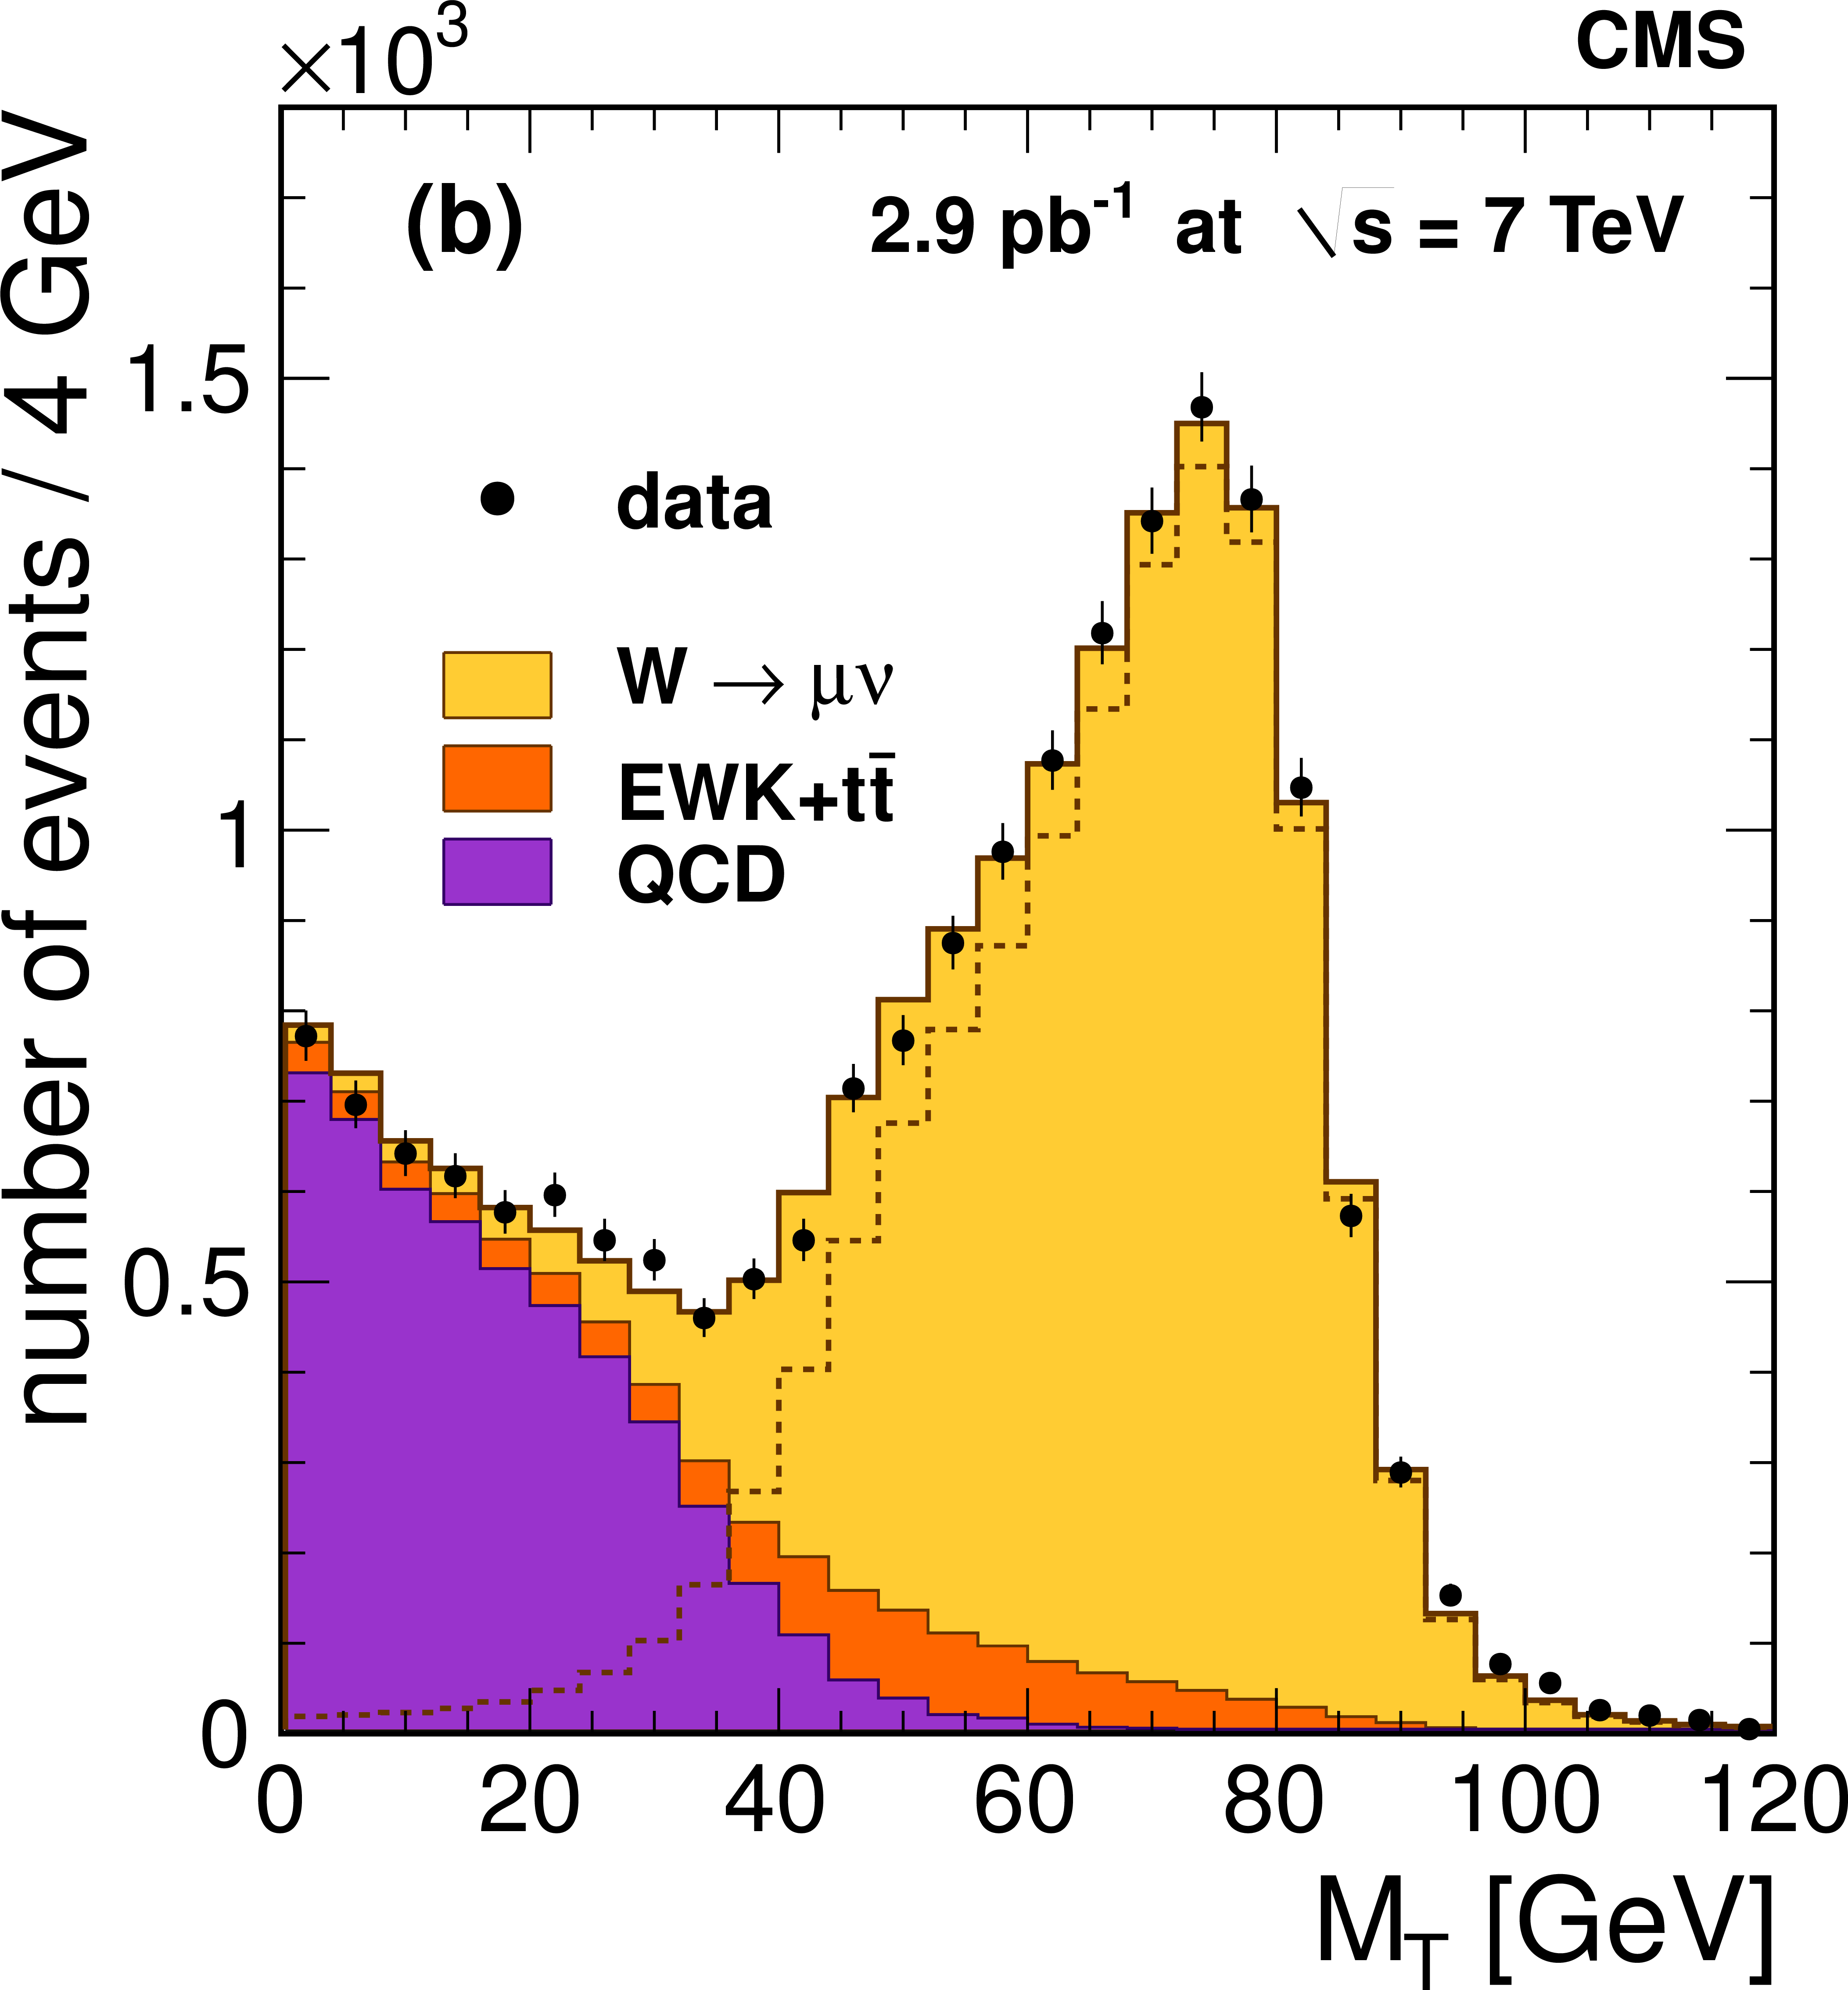
\includegraphics[width=0.45\textwidth]{figs/overview_mt2/w_transverse_mass.png}
    \caption{Transverse mass of the muon-\vMet system from a CMS measurement of the $W$ production cross section \cite{CMS:w_prod}.
      The transverse mass has a rough upper bound at $M_W=80\GeV$, limited by experimental resolution.
            }
    \label{fig:w_transverse_mass}
  \end{center}
\end{figure}

Computing the transverse mass of a decaying SUSY particle would be useful in distinguishing signal from background, since they tend to be much heavier than
SM particles that make up the background. However, the SUSY particles are \emph{pair-produced}, and computing the transverse mass 
of each system is not possible because it is not possible to resolve the \vMet vector into components from
each invisible particle. An example of this is the SUSY bottom squark pair production shown in 
Fig.~\ref{fig:example_susy_feyn} (right). Each bottom squark decays into a b quark, which appears
as a jet in the detector (potentially b-tagged), and a neutralino, which is invisible.

Absent this information, the best we can do is to try \emph{all possible partitions} of the \vMet vector
and choose the one that gives the weakest $M_\mrm{T}$ bound. This minimized quantity should be bounded above
by the mass of the pair-produced parent particles.
So, following \cite{mt2_def}, we define
\be
\mttwo = \min_{\vSS{p}{\mrm{T}}{X(1)} + \vSS{p}{\mrm{T}}{X(2)} = \vMet}
\left[\max\left(M_\mrm{T}^{(1)},M_\mrm{T}^{(2)}\right)\right],
\ee
where (from Eq.~\ref{eq:mtlong})
\be\label{eq:mti}
M_\mrm{T}^{(i)2} = m_{\mrm{vis}(i)}^2 + m_X^2 + 
2\left(E_\mrm{T}^{\mrm{vis}(i)}E_\mrm{T}^{X(i)} - \vSS{p}{\mrm{T}}{\mrm{vis}(i)}\cdot\vSS{p}{\mrm{T}}{X(i)}\right)
\;\;(i=1,2),
\ee
vis$(i)$ represents the $i^\mrm{th}$ ``visible'' system, $E_\mrm{T}^{X(i)}$ and $\vSS{p}{\mrm{T}}{X(i)}$ are the assigned transverse energy and momentum of each invisible particle, 
and $m_X$ is the mass of the invisible particle. The maximum of $M_\mrm{T}^{(1)}$ and $M_\mrm{T}^{(2)}$ is used, since if
the correct momenta are chosen then \emph{both} should be bounded above by the parent mass.

A couple of complications arise when trying to practically implement this. First, there are typically more than two visible objects
in an event (either the event is accompanied by ISR or pileup jets, or the decay cascade naturally produces more than one visible
object. For example, gluino decay into top quarks, illustrated in Fig.~\ref{fig:example_susy_feyn} (left), produces multiple jets per
decaying gluino). If the original pair-produced particles are produced back-to back, the visible systems tend to be in opposite
hemispheres. So before computing \mttwo, all jets in the event are clustered into two \emph{pseudojets} following the algorithm
described in Ref.~\cite{CMS:tdr_ii}, Section 13.4, and these pseudojets are used as the two visible systems. 
First, two initial seed axes are chosen. In this analysis they are chosen
by identifying the two jets that have the largest dijet invariant mass. Next, other jets are associated to one of these axes
according to a clustering criterion. Here we use the minimal Lund distance, meaning that jet $k$ is associated to hemisphere
$i$ rather than hemisphere $j$ if
\be
(E_i-p_i\cos\theta_{ik})\frac{E_i}{(E_i+E_k)^2} < (E_j-p_j\cos\theta_{jk})\frac{E_j}{(E_j+E_k)^2},
\ee
where $E_i$ and $p_i$ are the energy and momentum of pseudojet $i$, and $\theta_{ik}$ is the angle between pseudojet $i$ and jet $k$.
After all jets are associated to one or the other axis, the axes are recalculated as the sum of the
momenta of all jets connected to a hemisphere. The association is iterated using these new axes
until no jets switch from one group to the other.

A second complication arises in choosing the mass terms in Eq.~\ref{eq:mti}. Computing the masses of
the two pseudojets ($m_{\mrm{vis}(i)}$) is possible, but mis-measured multijet events with large pseudojet masses
may give rise to large \mttwo, eliminating some of the discriminating power of the variable. Setting
these pseudojet masses to 0 is found to further suppress multijet events while maintaining signal sensitivity.
The invisible particle mass, $m_X$, on the contrary is an unknown parameter and could not be set to its
proper value even if desired. It is found that setting $m_X=0$ is sufficient in maintaining discriminating power.
Hence, in this analysis both mass terms in Eq.~\ref{eq:mti} are set to 0 when computing \mttwo.

As discussed in Sec.~\ref{sec:mt2_backgrounds}, a big challenge in hadronic searches is the huge cross section
for QCD production of multijet events at the LHC. While requiring large \ptmiss suppresses much of this, there is still
a significant contribution from events with \ptmiss from mis-measured jets. The \mttwo variable allows further suppression
of these events, by taking advantage of the different event topologies between signal and mis-measured multijet events.

This is illustrated in Figs.~\ref{fig:inclusive_mt2} and \ref{fig:metmt2}.
Fig.~\ref{fig:inclusive_mt2} shows distributions of \mttwo for signal and background after an inclusive selection,
while Fig.~\ref{fig:metmt2} shows 2D distributions of \mttwo vs. \ptmiss separately for signal and QCD multijet events.
In SUSY events, the large mass scale of the produced sparticles and acoplanarity of the visible objects tends to concentrate
the events in the high-\mttwo region (\mttwo follows \ptmiss quite closely). On the contrary, mis-measured multijet events
populate the low-\mttwo region regardless of \ptmiss or jet \pt, since they tend to be ``back-to-back''.
Electroweak backgrounds have larger \mttwo tails than does QCD, since they contain real missing energy from neutrinos.
Because of this, after requiring high \mttwo, QCD multijet events become a sub-dominant background in all signal regions.


\begin{figure}[ht]
  \begin{center}
    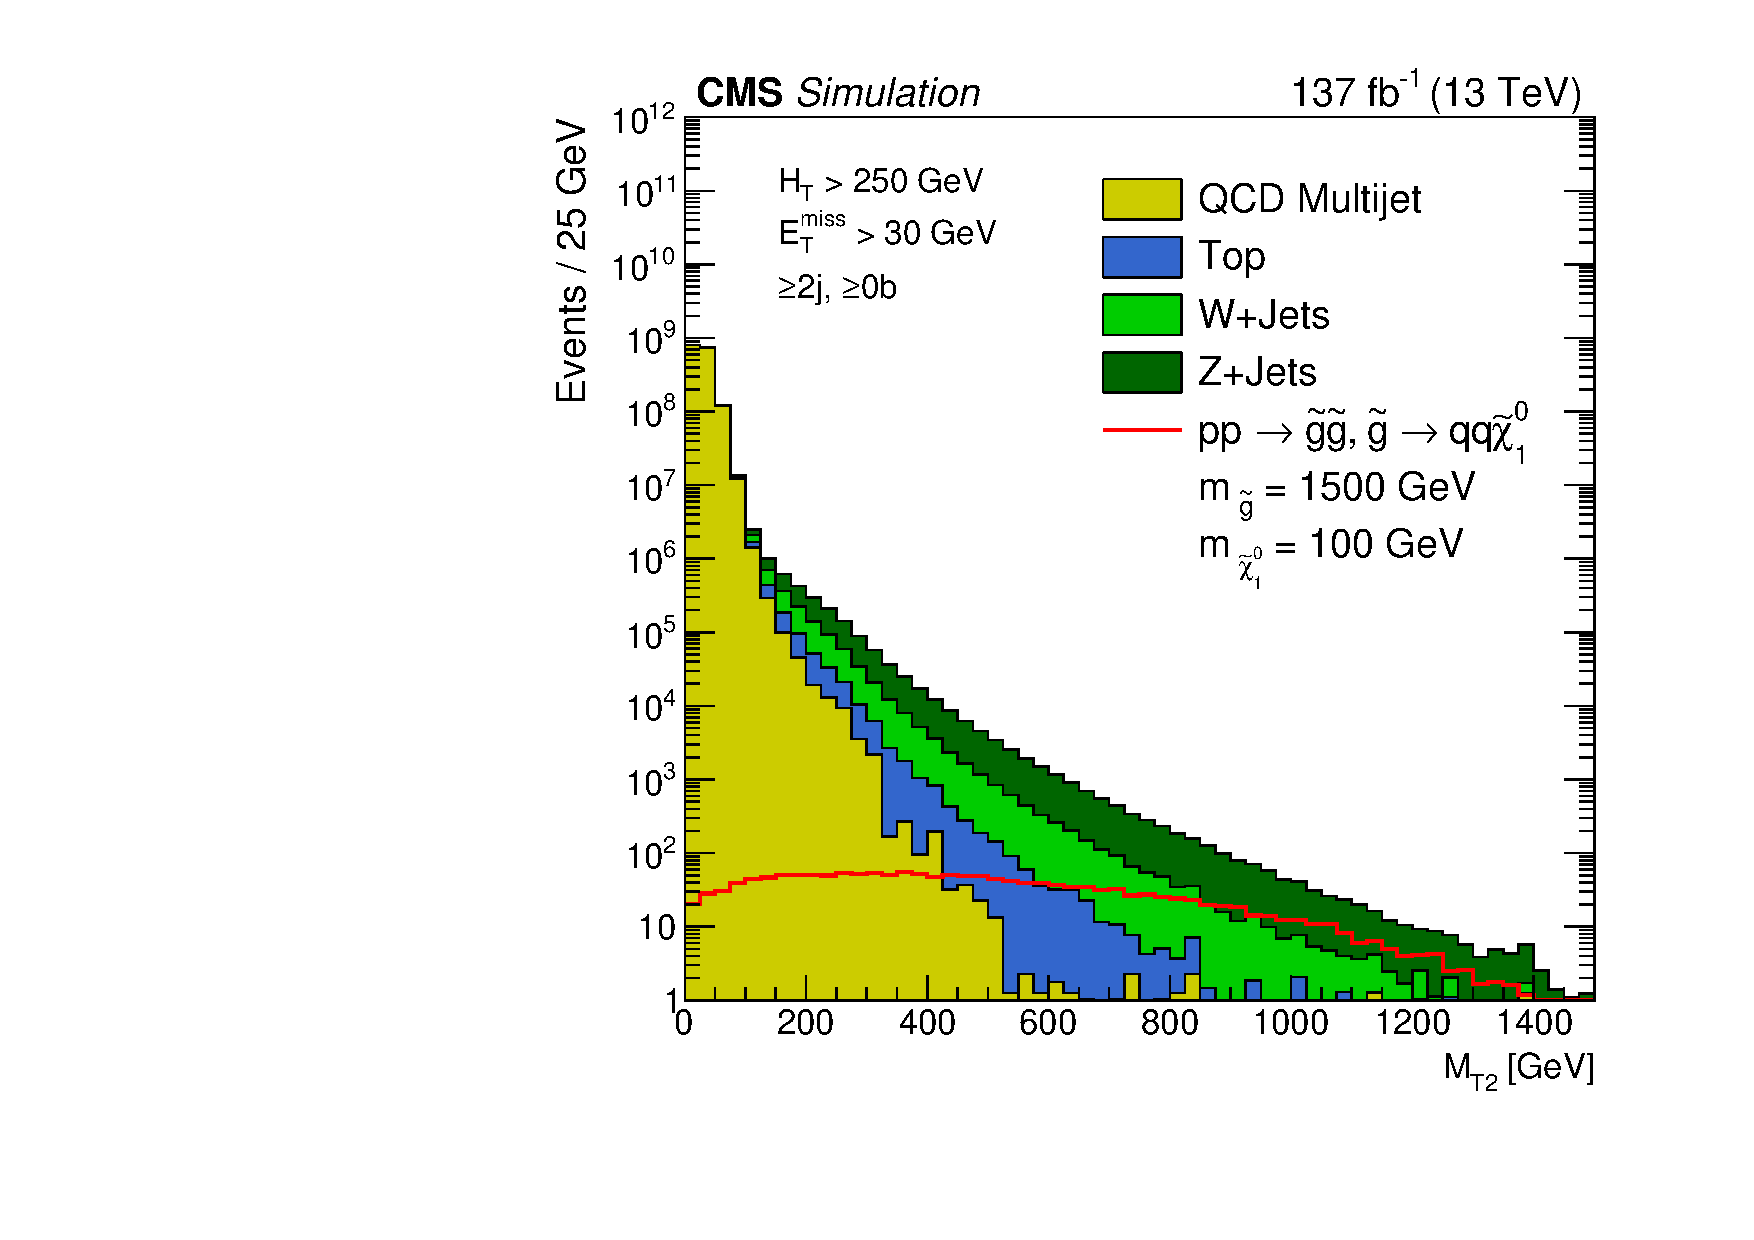
\includegraphics[width=0.50\textwidth]{figs/overview_mt2/inclusive_mt2.pdf}
    \caption{\mttwo distributions for an example signal and backgrounds after an inclusive selection of $\Ht>250\GeV$, $\ptmiss>30\GeV$, and $\Nj\geq2$.
      The signal shown is gluino pair production where each gluino decays to two light-flavor quarks and a neutralino, with 
      $m_\gluino=1500\GeV$ and $m_\lsp=100\GeV$.
      The QCD multijet background falls rapidly with \mttwo, while signal extends out to large values. The electroweak backgrounds
      have larger tails, since they contain true \ptmiss, but some discriminating power remains.
            }
    \label{fig:inclusive_mt2}
  \end{center}
\end{figure}

\begin{figure}[ht]
  \begin{center}
    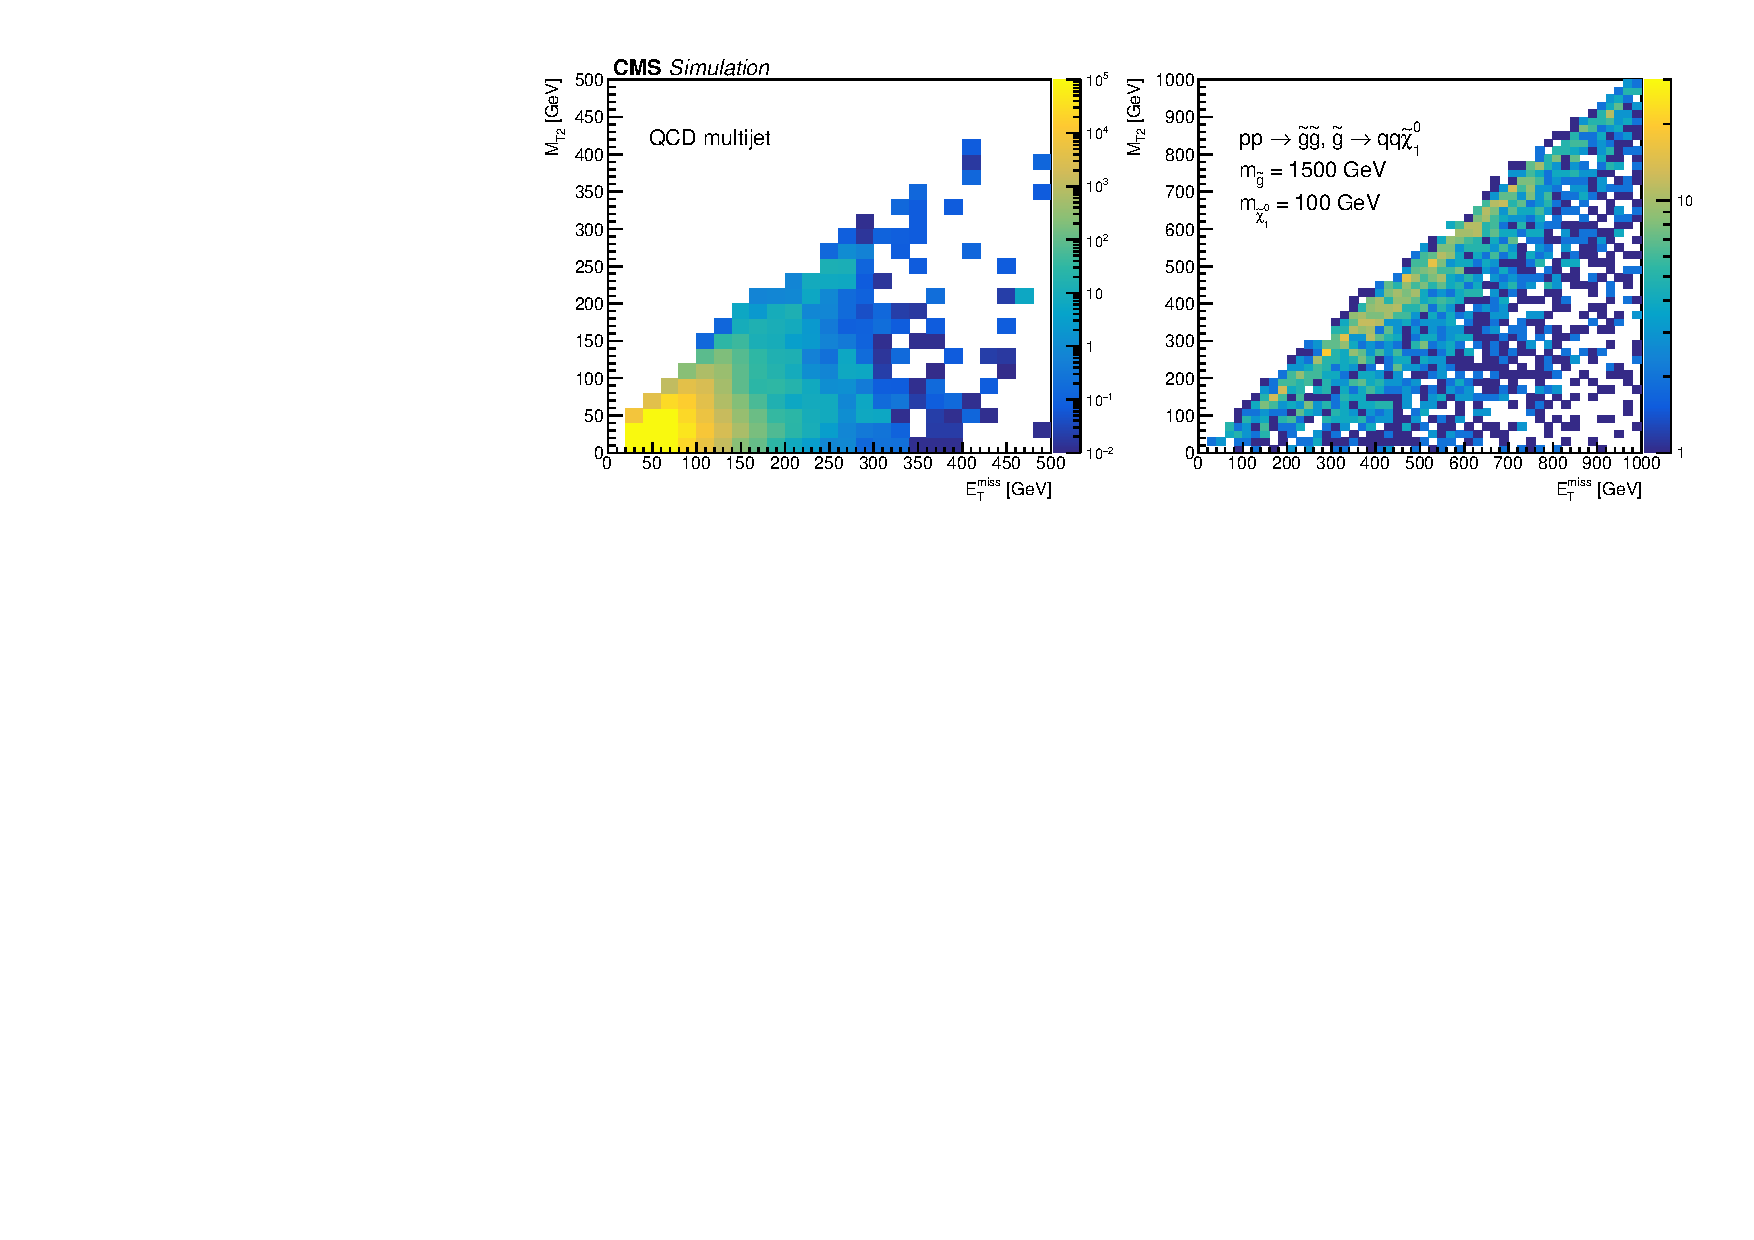
\includegraphics[width=0.98\textwidth]{figs/overview_mt2/metmt2.pdf}
    \caption{Distributions of \mttwo vs. \ptmiss, for QCD multijet events (left), and gluino pair production (right).
      For signal, $\mttwo\sim\ptmiss$, while for background, \mttwo tends to be much smaller than \ptmiss.
            }
    \label{fig:metmt2}
  \end{center}
\end{figure}
